\chapter{Background}
In this chapter I will present related work in this field. I will present different data acquisition systems, software analysis tools and openMNGlab which is an integral part of this thesis.\\
\begin{comment}
-Data acquisition systems: Spike2, Dapsys, OpenEphys\\
-Software analysis tools FieldTrip, Elephant, openMNGlab\\
-Neo package (included in section about openMNGlab)\\
-possible inclusion and cooperation with other software, such as elephant in openMNGlab context\\
\end{comment}
%TODO:\\
%-change the order of the topics:\\
%-order like in the analysis pipeline: data acqusition, analysis tools, openMNGlab\\
%rewrite transitions in particular and probably also the whole text\\
%-Available spike analysis frameworks \\
%-fieldtrip \\\
%-elephant \\
%-Why they are not sufficient \\
%-problem with the relays? maybe windows updates 
%-openMNGlab as a solution \\
%-acquisition frameworks we need to handle \\
%-Current status of openMNGlab, including Neo \\
%-go into detail on different data acquisition softwares \\
%-Dapsys, OpenEphys, Spike2 \\
%-why does dapsys not work in the future \\

\section{Data acquisition} 
A data acquisition system is a combination of software and hardware components that work together in order to control inputs and record data from different subjects. Whenever researchers want to record electrophysiological data, these system are used.
There are three systems that I will describe here and that should be compatible with OpenMNGlab. These systems are Spike2, Dapsys and OpenEphys.

\subsection{Spike2}
%“Spike2 is a multi-channel continuous data acquisition and analysis package”( https://ced.co.uk/products/spkovin) produced by Cambridge electronic design limited. \\
%-Used for the experiments I am analysing by Roberto \\
%-records data in multiple channels \\
%-channel for raw signal \\
%-channel for mechanical force \\
%-channel for event markers \\
%-channel for temperature (not used by me) \\
%-channel for comments (used for marking when chemicals are applied) \\
%-spikes can be separated into own channels (done by experimenters) \\
%-software offers a graphical representation of the data \\
%-channels are separated \\
%-was used for confirmation of what the data should output in terms of basic quantifiers \\
%-can export csv files from the data \\
%-has direct importer in openMNGlab \\
Spike2~\cite{spike2} is a data acquisition and analysis software produced by Cambridge electronic design limited for electrophysiological data. It is a flexible tool that can be used in different ways.

\begin{figure}
	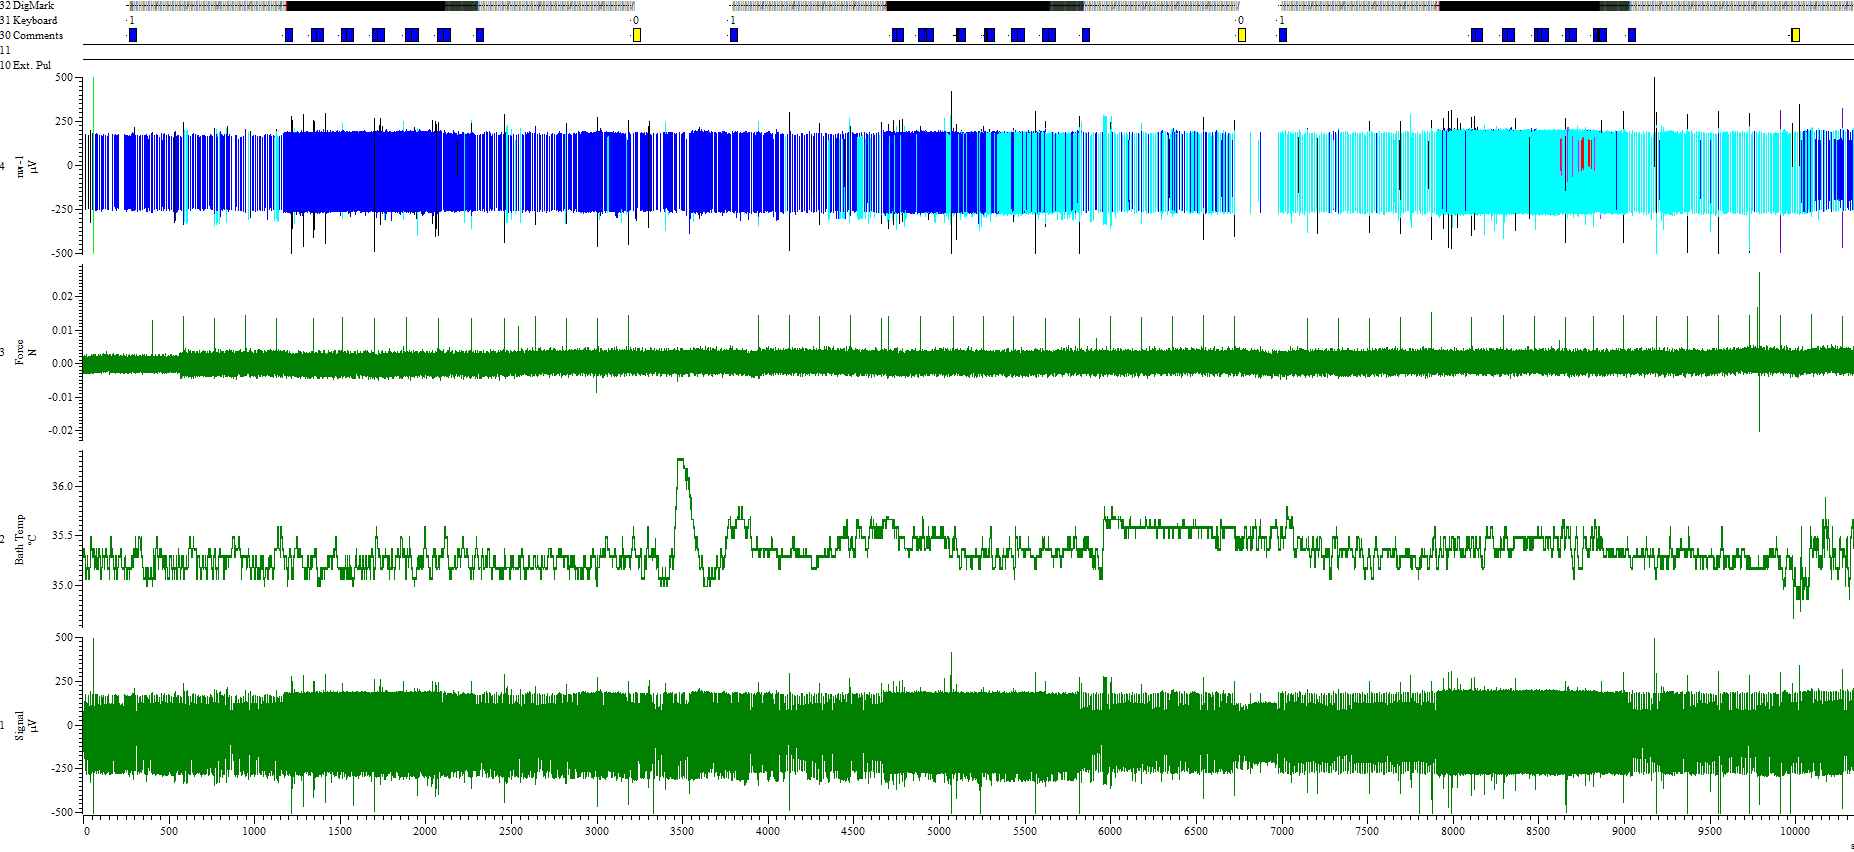
\includegraphics[width = \textwidth]{src/pic/Spike2_screenshot}
	\caption{Typical mechanically and electrically stimulated recording in Spike2}
	\label{fig:spike2}
\end{figure}

The software can record multiple channels simultaneously. An example screenshot from a recording can be seen in figure~\ref{fig:spike2}. This depicts a typical recording used for analysis in this bachelor thesis. The recording contains data from nerve fibers of rat cranial dura mater. The nerve fibers were stimulated using a mechanoelectrostimulator applying electrical and mechanical stimulation. I will now describe the different components of the software.\\

\begin{figure}
	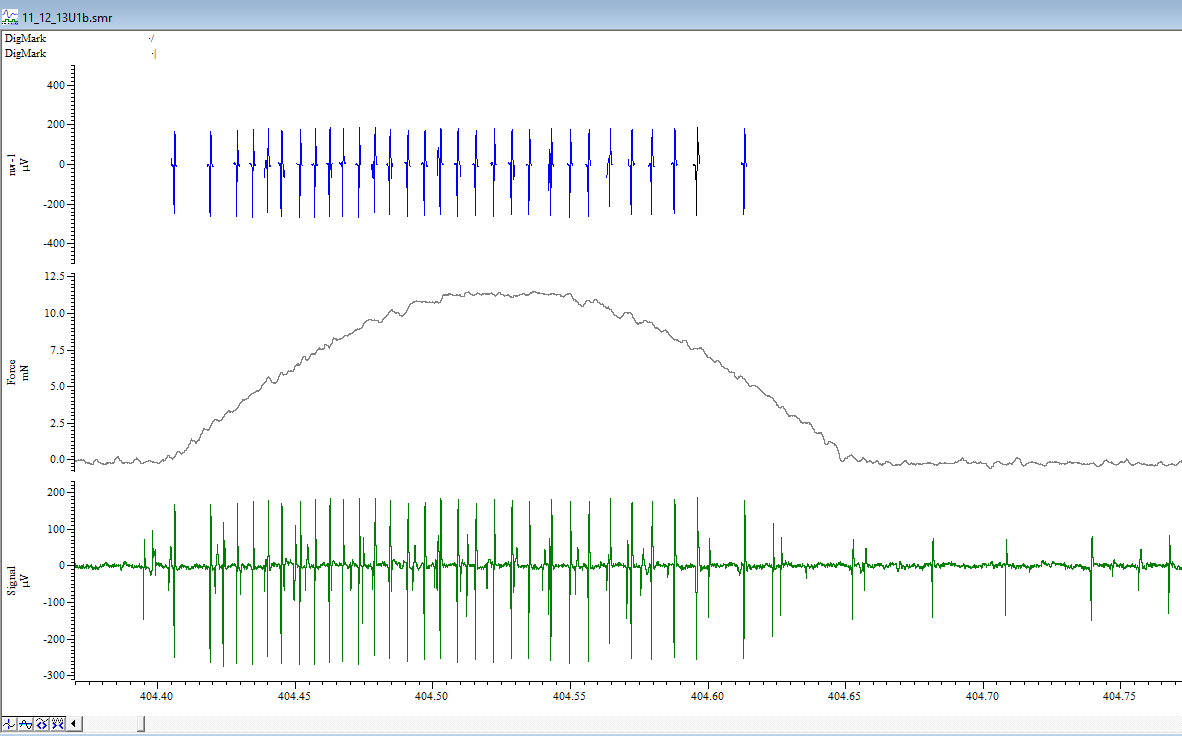
\includegraphics[width = \textwidth]{src/pic/Spike2_spike_train}
	\caption{A single spike train in spike2}
	\label{fig:spike_train}
\end{figure}

First of all it contains the recorded raw signal($\mu$V) at the bottom in channel 1. The next channel contains the temperature during the recording in degrees celsius. In this example it fluctuates between 35°C and 36.5°C. In channel 3 we can observe the mechanical force that was applied to the nerve fibers. In figure~\ref{fig:spike2} we can see the mechanical force spiking whenever a mechanical stimulation occurs to evoke a spike train. \\
For this experiment we want to collect the data of single nerve fibers. However, it is difficult to record just a single fiber, when recording in vitro. This is why in this experiment spike templates are applied to the raw signal to sort spikes to specific fibers. These filtered fibers are then displayed in so called wavemark channels. In this example channel 4 is such a channel, where only specific action potentials are filtered. The filtering process is done by the experimenters and is based on certain features of the action potential shape.\\
The electrical and mechanical stimulus events are always stored in channel 32, which is the topmost channel in figure~\ref{fig:spike2}. The two different stimuli are denoted with a different symbol in this channel. Additionally there is a channel containing comments regarding the experiment. Comments can represent the experimental protocol and are given by the experimenters. In this example there are comments denoting a change in electrical stimulation frequency. In other experiments for example, these could also denote the application of certain chemicals towards the recorded subject.

A more detailed view of a single spike train can be seen in figure~\ref{fig:spike_train}. Here the difference in electrical and mechanical event markers in the two topmost channels can be seen. Mechanical markers are represented by a slash, while electrical markers are represented by a vertical line. Another thing that can be seen here is the channel containing only the spikes. This channel is ideal for the extraction of the spikes for later analysis as there is no noise in the channel anymore and the spikes can also be interpreted as simple events with a timestamp.

\subsection{Dapsys}
%“DAPSYS is a combined hardware and software system designed for real-time acquisition and display of data and synchronous %control of stimulators.” (http://www.dapsys.net/) \\
%-Used by Barbara for her experiments \\
%-used for mng-experiments with human patients \\
%-also has a graphical representation of the data \\
%-has importer in openMNGlab \\
%-needs to export specific templates as csv for the importer to work \\
%-Dapsys has problem in the future \\
%-it gets harder to set up experimental protocols \\
%-maybe it has something to do with newer windows updates \\
%-that means this will probably not be used much in the future \\
%http://www.dapsys.net/rd_article/rd_article.html

The second data acquisiton package that our analysis software system needs to support is called Dapsys~\cite{dapsys}. It is a hardware and software system that can record and analyze electrophysiological data from animal or human sources and has been mainly used for studying the peripheral nervous system. It has been in development for over 30 years since its earliest version and thus has a great history of usage in the field. The idea behind the conception was to build a system that could control stimulators and simultaneously acquire the data in real-time and display the data~\cite{dapsysArticle}.\\
Dapsys offers the capabilities of path tracking and comes with the benefit of much data being available from experiments conducted with the Dapsys software. It was developed for animal experiments originally and then later adapted to also handle human MNG data. As is the case for Spike2 it also comes with a visual representation of the data which can be seen in figure~\ref{fig:dapsys}. This graphical interface works real time while recording the data.\\
\begin{figure}
	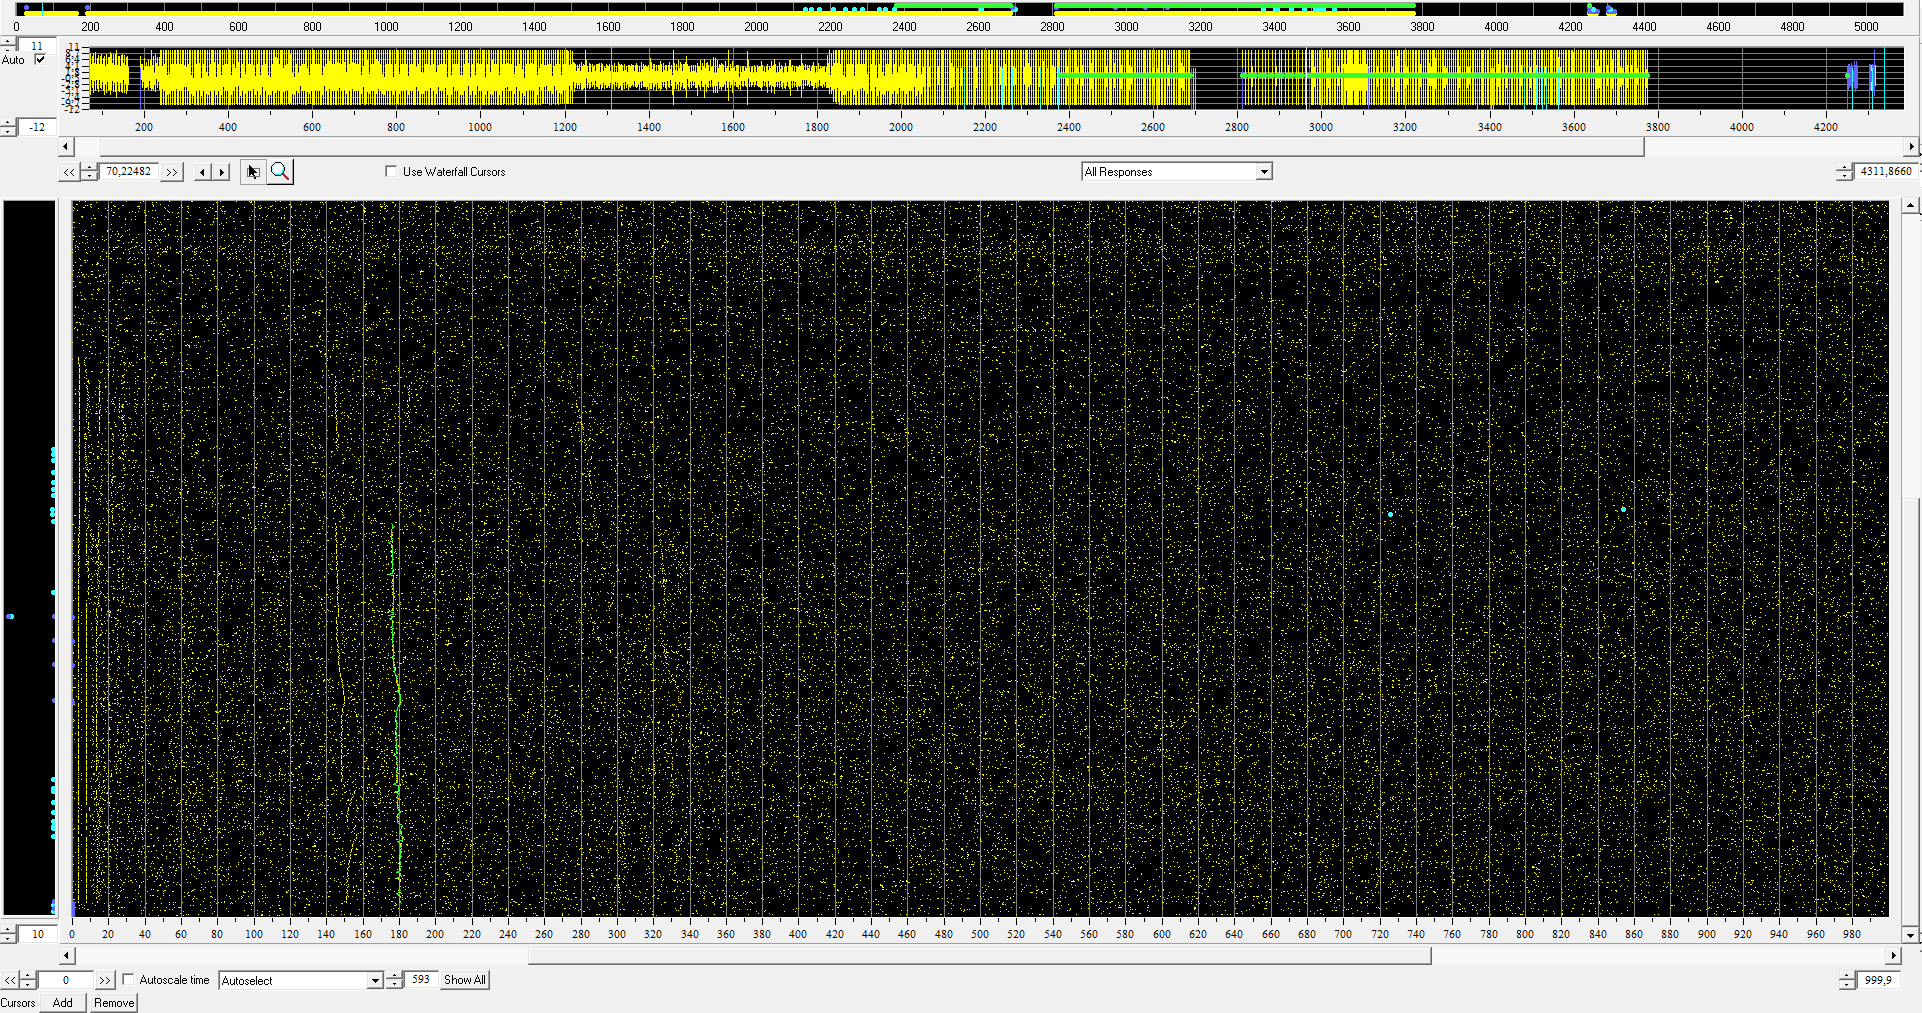
\includegraphics[width = \textwidth]{src/pic/Dapsys_sc}
	\caption{Screenshot of a recording in Dapsys}
	\label{fig:dapsys}
\end{figure}
%All versions of Dapsys are highly specialized
%The version of Dapsys used in the experiments from Barbara Namer is specialized for microneurography and was configured in cooperation with Brian Turnquist.\\


\subsection{OpenEphys}
%OpenEphys \\
%-open-source electrophysiology \\
%-based in Cambridge, Massachusetts \\
%-Used in experiments in Bristol cooperation \\
%OpenEphys is an open-source electrophysiology data acqusition software from a nonprofit based in Cambridge, Massachusetts. Its aim is that in the future neuroscientists can choose the right tool for their job and that there are many tools available. This is best accomplished by providing open-source solutions.\\
%They provide a platform where researchers can individually choose their own experimental setup from a number of different open-souce and other components.
%OpenEphys is used by one of the collaborators of IMI in Bristol.

The last data acquisition system I want to focus on is called OpenEphys~\cite{openEphys}. It is an open-source electrophysiology data acquisition system originally developed by a nonprofit based in Cambridge, Massachusetts. It sets a big focus on modularity and flexibility so that it can fit many different needs from a variety of users.\\

The idea behind OpenEphys came after an increased popularity of closed-loop experiments in neuroscience, in which the results of the recorded system has an influence on the system itself. With proprietary systems it is difficult to share the details of such experiments and to replicate them. The introduction of OpenEphys, an open-source system is supposed to make it easier to develop and share analysis and details of such closed-loop experiments.\\
OpenEphys makes use of inexpensive open-source hardware such as Intan chips~\cite{openEphys} to make it easier for small labs to get started with analyzing electrophysiological data. The heart of the software is a plugin-based graphical user interface (GUI). Here the user can add different modules to the processing pipeline such as modules for communicating with the hardware or modules for analyzing the data.\\
Different labs often have widely varying sets of requirements towards data analysis and therefore data acquisition systems. At the start of a project they are confronted with the question of whether to use a proprietary system or develop their own systems, which will result in much more effort before the real work can begin. Proprietary systems also often come with very limited customization possibilities, which makes it harder to fit the system to the users needs. This is where OpenEphys comes in with its plugin-based software. It is designed so that everyone can mix and match the processing modules and end up with the exact analysis pipeline that they require. In addition to a wide array of already available processing modules, it is possible to develop your own modules that fit seamlessly into the structure of the system. OpenEphys is completely developed in C++ and based on a library for audio applications. This makes it easy to develop new modules by making use of the class inheritance capabilities of C++.\\
OpenEphys comes with many advantages such as low cost, transparency and flexibility due to the modularity, but there are also drawbacks of using the system. The start is a little harder than in proprietary systems, where there is often a straight forward way of getting started with your first experiments. The modular nature of the system might also effect the performance of the analysis, which is why commercial systems might be a better choice, if they fit the analysis needs.\\
OpenEphys is a system which is used by an associated research group in Bristol, who should also be able to incorporate OpenMNGlab in their analysis.

\section{Common Spike Train Analysis Methods}
When reading the literature regarding spikes, spike trains and their analysis I also looked at what the most common analysis methods are. I found that there is not one definite way to analyze a spike train, but that different papers use different quantifications and statistics, depending on their set of experimental data.\\
In the early literature attempts were made to model the probability of spikes appearing at specific times in a spike train~\cite{spikeGeneral}. The most common model for this is the poisson model, which uses a poisson process to calculate the probability of spike distribution.
The book by Rieke et al.~\cite{rieke1999spikes} also proposes a raster plot to visualize the spike data from multiple trials with the same conditions. The response to the same stimulus did not elicit an identical response over many trials. From the time data that is used to plot this, they also plotted a post stimulus time histogram. For this they counted the average number of spikes in bins of a specific time (10ms). This gives the firing rate as a function of time.\\
The reference paper from Uebner et al.~\cite{roberto} that produced the data that this thesis is about used another quantifier. In this paper the effect of background stimulation on a mechanical stimulus that did not change was studied. To quantify this effect, they used the peak firing frequency that averages the 5 highest instantaneous frequencies of spikes per spike train. This was the main indicator for changes in the spike trains and therefore I have also incorporated this into my analysis.


\begin{comment}
Poisson process?
Fano factor
raster plots
post stimulus histograms with buckets for the spikes per time interval

Interspike interval distribution is use to look at the time between two successive/adjacent action potentials in a spike train.
Spike train autocorrelation function describes the distance between spike for a whole spike train and can show the oscillations.

I did not find THE one way to quantify spike trains that was mentioned in every source. Most stuff is pretty individual and tailored to the specific use case and experimental data.
most papers try to look at how to model a spike train. The most common way to model spike trains is with a poisson process

Spike trains start from a point and then cover a period of time. In the general literature, there are a few ways to analyze spike trains.\\
Poisson model: there are a few possibilities that describe how to model a spike train. This gives us information on the probability of spikes appearing at specific times after the spike train has started~\cite{spikeGeneral}. One basic quantifier for spike trains described in Spikes: ... is a raster plot. This plot shows a dot for every spike occurring. This is useful for describing an experiment with multiple trials, that show the same response. Furthermore there is also the post stimulus time histogram, short psth, which puts the spikes from the raster plot into buckets to show a distribution of the spikes over time for many trials.\\
In~\cite{spikeGeneral} there is also the mention of interspike intervals. This measures the time between two consecutive spikes and can also be used to describe spike trains.\\
There are, however, no really specialized quantifiers that are described in literature that are the go to numbers for spike trains. Many experiments cover different problems that produce different sort of spike trains and therefore, there are also many different characteristics that might be important for each experiment.
\end{comment}
\section{Spike Train Analysis Tools}
I will now present two software tools for microneurography analysis, before focusing on OpenMNGlab.


\subsection{FieldTrip}
Fieldtrip~\cite{fieldtrip} is a MATLAB toolbox developed at the Radboud University,  Nijmegen,  the Netherlands and offers a wide variety of analysis functions.  It can analyze MEG, EEG, and iEEG and is an open-source software that has been in development since 2003. Its main strengths lie in the analysis of invasive and non-invasive electrophysiological data. It provides over 100 high-level and 800 low-level functions that can be used both by experimental users as well as developers. It does not feature a graphical user interface, but instead focuses on providing direct access to the high and low-level analysis functions that can be used in the command line or in scripts.  This increases flexibility and is done because FieldTrip is not meant to be an application but a set of tools that can be mixed and matched for different requirements.
With this approach the user needs to be familiar with MATLAB before starting their analysis, but after a potential initial time invest the flexibility of this approach yields great advantages.
The analysis functions are meant to be combined and used as a sort of analysis protocol, where the output of functions is used to compute the next results. 
An example pipeline is lined out in the paper~\cite{fieldtrip}. The first step after loading a data set is to choose a data segment to be analyzed by setting the boundaries of the segment. In order to free the data from noise and artifacts that could compromise the analysis. FieldTrip provides the corresponding functions for automatic removal of artifacts. As a next step the user can run a preprocessing function that loads the specified data into the MATLAB workspace and readies it for further analysis. Then the user can choose which specific analysis they want to perform. There is also the possibility of source reconstruction to get a visual representation of the source of the data.\\
An important feature of FieldTrip is the ability to save and reuse intermediate results. After each step in the analysis there is the possibility to save the current results for later use before further altering the data. This can be useful in many situations where the user wants to retrace certain steps in the analysis.\\
For visualization of results users can make use of standard MATLAB functionalities to plot the numeric results of FieldTrip analyses.\\
As an open-source software FieldTrip is also meant to be contributed to by developers who see opportunities for improvement. As opposed to other GUI-using software FieldTrips focus on having the direct access to functions lends itself to development and contributions from various different experts, which only enhance the product.

This software package is very useful and widely used in the field, however it does not lend itself to our specific needs.
The main problem with this software is its programming language. It is a MATLAB toolbox, however it would be preferred to use a software package in python or another programming language that slots better in the already existing structure that is used at the chair for medical informatics.  

\subsection{Elephant}
Elephant~\cite{elephant18} is a python module which offers high-level analysis functions for electrophysiological data.
It also features functions that are designed specifically for spike trains. It does provide functions for high-level analysis, but is lacking when it comes to very basic functions and quantifiers for spike trains. 
Its focus on highly specified analysis tools makes it not viable in our use case. For the use in this thesis I want to start with the basic signal from the spikes. Then the goal is to try and quantify spike trains, starting with basic measures as number of spikes for example. This is not something that Elephant provides. Once this ground level analysis is done we can think about the more advanced analysis provided by such tools as Elephant.

\section{openMNGlab}
The previously presented analysis tools have their uses in different use cases, but are not suitable for this thesis for a variety of reasons.
There are multiple data acquisition systems that are used at the institute of medical informatics(IMI) that each produce different file formats. The three main systems that need to be handled are the previously described Spike2, Dapsys and OpenEphys. \\ 
We need a tool that that has the capability to load files from these different data acquisition systems, put them in a compatible format and analyze them further.  FieldTrip does not offer these kinds of capabilities as well as it being a MATLAB package, which would not be ideal for fitting into the rest of the analysis systems at IMI, which are based on python. Elephant is a python tool, but is lacking the importing tools that would be required for the software solution.  \\
For this reason IMI has started to develop their own software framework in python called openMNGlab~\cite{schlebusch_openmnglab_2021}.  This framework aims to provide a solution for dealing with different experimental file types and combine them into a single usable format.  In addition it aims to provides analysis capabilities for microneurography data. \\
OpenMNGlab was started as a project of IMI and was initially developed by Fabian Schlebusch who developed openMNGlab 1.0 and set up the basic structure and developed the importers necessary for the file formats that we require. \\
However, the 1.0 version of the framework, being an early version,  still came with a few issues. The biggest one being the functionality of the importers. The software was not capable to import the raw experimental files from the Spike2 and Dapsys systems. An additional extraction step was required to create csv files that could then be imported into openMNGlab. \\
In the beginning the goal of having everything in one format was not a priority compared to getting a working analysis for the different files. This resulted in analysis functions that were not usable for every recording that should have been analyzed.\\

\subsection{Neo}
To help with these issues, Neo~\cite{neo14}, a python package for representing electrophysiological data, was integrated into openMNGlab. This package provides a way to model electrophysiological data in a hierarchical structure that becomes the new basis of openMNGlab. From now on the data will be modelled with Neos hierarchical structure. 
Neo also comes with built in importer functionalities for many different files formats and templates to develop importers for new file formats.  These importing tools help to solve the previous importing issues in openMNGlab. This enables us to import raw Spike2 files directly, which makes the analysis process much less cumbersome as one step in the analysis pipeline gets eliminated. 
When using the importers provided either through Neo directly or via its templates, the imported data immediately has a uniform structure, regardless of its origin. \\
Neo does not provide analysis on its own, but we can now base all of our analysis on the structure it provides (that will from now on be referred to as Neo structure). \\

%With this bachelor thesis I aim to provide some ideas for analysis functions for openMNGlab as well as put some thought into the software engineering aspect of the framework.





%At IMI there are people who work on varying aspects of MNG data analysis such as analyzing the response latency to electrical stimulation or analyzing the nerve activity in response to certain chemicals. I am focusing on analyzing spike trains occuring in mechanically and electrically stimulated nerve fibers.\\

%In the end FieldTrip and Elephant offer good solution for slightly different use-cases, but are not a perfect fit for the analysis of microneurography data at the Institute of medical informatics. They are, however, a good inspiration for what should be included in such a software framework. In the case of Elephant, since it is also a python module and also makes use of the Neo structure, it could make for a good addition of more high-level analysis functionalities in the future.

\subsubsection{Cooperation with other software}
The importer for Spike2 files is already developed with the help of the Neo package and therefore many experiments that were recorded with the Spike2 software can be analysed using the framework. The same can be said for OpenEphys files, since Aiden Nickerson, a collaborator in Bristol, has implemented a corresponding importer.
OpenMNGlab already features an importer for Dapsys recordings, which makes many experiments conducted with this system readily available for analysis.
The difference to Spike2 however, is that the importer can not deal with the raw recording files, but requires an extra step from the user. We need to export the raw data we want to analyze as csv files from the Dapsys software, before we can import them into openMNGlab. This process is especially cumbersome when dealing with a larger number of recordings. In the future the importer functionality of openMNGlab should be improved, so that it works on the raw Dapsys files in order to make the analysis workflow easier. This is especially useful since there are many experiments recorded with Dapsys that we would like to analyze.\\

The Matlab functions offered by FieldTrip, while similar from a functionality point of view are not very compatible with our python environment. We can, however, take a look at the functions of FieldTrip and take inspiration for similar functionality in openMNGlab.
The case is different for Elephant. While the functions may be too advanced for the analysis done in this bachelor thesis, they might become useful in future work.  With Elephant also being a python module, the compatibility to openMNGlab is much higher and the possibility of combining functions from each package in the future might be worth keeping an eye on. 



\begin{comment}
Neo:\\
brings a data structure\\
importers or at least templates for importers

As mentioned before, Neo is the basis of openMNGlab when it comes to the structure of the data. It provides a common ground for electrophysiological data from different sources. It 
Because it is meant to be used in conjunction with many different file formats, it already comes with importing functionalities for a couple of formats. In addition to the already available importers, Neo provides the tools to write new importers for file formats which are not already supported. These templates are the basis of the importers in openMNGlab.
\end{comment}


\section{Experimental Data}
This thesis is based on the analysis of Uebner et al.~\cite{roberto}. In this paper they analyzed the activity dependent axonal conduction velocity slowing in slowly conducting meningeal afferents. They studied the effect of preceding action potential activity on mechanical stimulus response.\\
The results show that there is a significant decrease in peak firing frequency after the fiber was previously electrically stimulated with a frequency of over 2 Hz.




 
\cleardoublepage
